\section{gm2Geane Error Propagation}
\label{sec:gm2Geane}


	As with any experiment, the physics of the simulation needs to be attuned to what we observe and the particularities of our detectors. This includes tuning errors and energy loss due to physical processes that particles experience within our tracker system. A quick summary of the relevant Geant4 source code and the changes that have been made will be given. Within every default install of Geant4, there is a folder with the name ``error\_propagation''. As mentioned in the \hyperref[sec:GeaneParamUtils]{GeaneParamUtils} section, this package propagates particles along their average trajectories within a Geant4 world including the magnetic field. Errors and average energy loss due to the presence of material is included, and there are a number of methods to calculate track parameters and errors within different reference frames.

	Within the ``error\_propagation'' folder there are a number of classes. Because some changes have been made to this Geant4 source code, several of these classes have been copied into the gm2tracker package and it's those classes that the Geane fitting has been linked to. (A quick aside - the code and physics described in this section are currently contained within the ``artg4'' package with the folder name ``gm2Geane,'' but will soon be moved into the ``gm2tracker'' package. I will write this section as if they are already in gm2tracker, but it's good to know this in case the change hasn't been made by the time the reader reads this document, or if the reader wishes to look at old versions of the code.) Because of the linking of those classes to further c++ header classes in the error propagation package, a further number of classes have been copied into this gm2Geane directory with the only changes being header file names. When examining this source code, one will need to look within both the gm2tracker/gm2Geane folder as well as the error\_propagation folder in Geant4 in order to get the whole picture. (All these classes of course link to other Geant4 source code dealing with transportation, geometry, etc.)

	Most of the file names are relatively self explanatory. ``gm2GeanePropagator,'' ``gm2GeanePropagatorManager'', and ``gm2GeaneRunManagerHelper'' all deal with the overhead and set up of the error propagation routines and aren't worth going into more detail about. It suffices to say that it's these classes that are instantiated within GeaneParamUtils.cc and where the base methods are called. There are then the classes ``gm2GeaneFreeTrajState,'' ``gm2GeaneFreeTrajParam,'' ``gm2GeaneSurfaceTrajState,'' and ``gm2GeaneSurfaceTrajParam'' which are derived from some simpler base classes. These deal with the track state and parameter information of the propagated track in the free system and whatever surface system one is working within. They have a number of methods for grabbing these errors, parameters, and matrices. Track errors and other matrices are created within the ``gm2GeaneMatrix'' and ``gm2GeaneSymMatrix'' classes, which are 5x5 matrices with units of GeV cm instead of the usual Geant default of MeV mm. It's important to be aware of this in order to convert these units in various parts of the fitting code. There are also a couple of classes related to the physics list, step limiters, and targets that Geant uses when performing the track propagation. 

	The most important class to understand is probably ``gm2GeaneFreeTrajState.'' The transport matrix is calculated within the long method ``PropagateError'' with the variable name ``theTransfMat'', which is then used to propagate the track error from one point to another. It's important to note that this transport matrix is only generated on a step by step basis, and is not saved from target to target. The calculation of this transport matrix (which is just a Jacobian from one curvilinear frame to another) is completed in reference \cite{jacob}. In the same file the errors on the track propagation are calculated within the methods ``PropagateErrorMSC'' and ``PropagateErrorIoni'' which calculate the error due to multiple scattering and ionization respectively. Note that there is no such method for the error due to bremmstrahlung, which is a rarer process with a larger randomization of energy loss. The Geant4 defaults for these errors are sufficient (but not perfect) for the tracking results so far, but will at some point need to be tuned. (The p-value distribution rises slightly towards 1 indicating an overestimation of errors.) Some basic attempts at error tuning were done using the path taken in Chapter 4 of reference \cite{Lavezzi} for the PANDA experiment, which recommends modifying both the multiple scattering error very slightly, and adding an extra term to the ionization errors for delta ray production in thin gaseous detectors. These quick studies with the constants given in that reference didn't result in much changes or improvements and so have been left commented out (but available) in the gm2Geane code. (The delta ray term can be modified to make the error infinitely large if one wishes.) When performing more detailed tuning studies, I highly recommend reading the relevant sections of Chapter 4 of reference \cite{Lavezzi} as it contains further derivations and explanations that are not included here.

	The class ``gm2GeaneSurfaceTrajState'' is one of our main hooks into the error propagation code for grabbing the errors and surface trajectory parameters. Those errors and parameters are then transformed to our preferred coordinate system as described in the \hyperref[sec:Coord]{Coordinate Systems} sections. Within this class the ``BuildErrorMatrix'' method calculates the relevant Jacobian to convert the error from the free trajectory state to the surface trajectory state as described in \cite{jacob}.

	Finally, there is the ``gm2GeaneEnergyLoss,'' ``gm2GeaneLossForExtrapolator,'' and ``gm2GeaneTablesForExtrapolator'' classes which deal with the energy loss of the particle as it is propagated within the Geant4 world. (These files were not originally in the error\_propagation directory but in other parts of the Geant4 source code.) The full path of function calls will not be included here, it suffices to say that when ``gm2GeanePropagator'' calls ``MakeOneStep'' the Geant4 stepping manager is called which then links to the Geant4 transportation and on to the physics calculations. This is done on a step by step basis with the physics list used to calculate the average trajectories of the particles. There is some information on the default energy loss relevant to our track fitting in reference \cite{energyloss} which is useful to understand. However it turned out that the default was including bremmstrahlung energy loss effects which consistently overestimated the energy loss of particles through our thin gaseous detectors. (Thanks to James Mott for confirming this.) In order to remove this effect, within the class ``gm2GeaneTablesForExtrapolator'' the brem additions to the energy loss were removed in the various methods, including ``ComputeElectronDEDX'' which is what is called when we propagate positrons. Once this was done, the reconstructed energy loss more closely matches truth, see Figure \ref{fig:bremComparison}. The simulated energy loss for a distribution of tracks within our detector can be seen in Figure \ref{fig:eLoss}, which is what we will expect in reality.

\begin{figure}[]
\caption{It was noticed during the course of debugging that the Geant4 error\_propagation routines were consistently removing too much energy on average from all tracks as they passed through the tracker during reconstruction. It was discovered that the Geant4 tables were taking out too much energy due to bremsstrahlung processes and it was decided to remove this effect. The left plot shows in a red the true particle momentum as a function of X distance through the tracker, and in black the reconstructed momentum before bremsstrahlung was taken out of the reconstruction for a single event. The differing slopes signify the problem. The right plot shows the same event but with bremsstrahlung taken out. Notice the scale change, and that the reconstructed momentum aligns much more readily with the truth.}
\centering
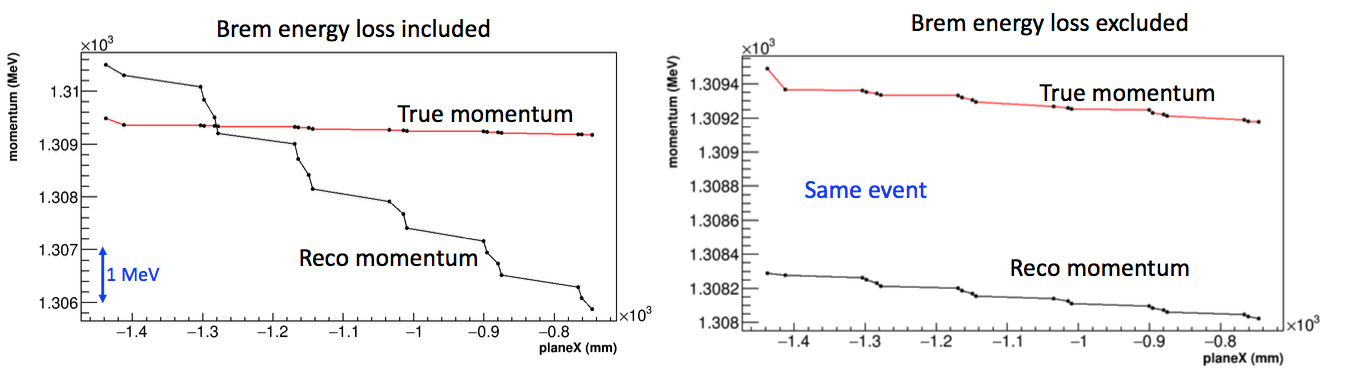
\includegraphics[width=1.0\textwidth]{bremComparison}
\label{fig:bremComparison}
\end{figure}


\begin{figure}[]
\caption{Shown here is the energy loss between the first and last hit in the tracker from simulation with the full physics list for a distribution of tracks. (Momentum magnitude difference.) Note that this is from event generation, and not from reconstruction. Sources of energy loss come from ionization and bremsstrahlung processes, which account for the long Landau tail running off to infinity. The distribution has a mean of approximately 220 keV and and peak centered at about 150 keV, which is reasonable for the material composition of our trackers and tracker gas. More than 50\% of the energy loss comes from the mylar walls of the straws as seen in the simulation.}
\centering
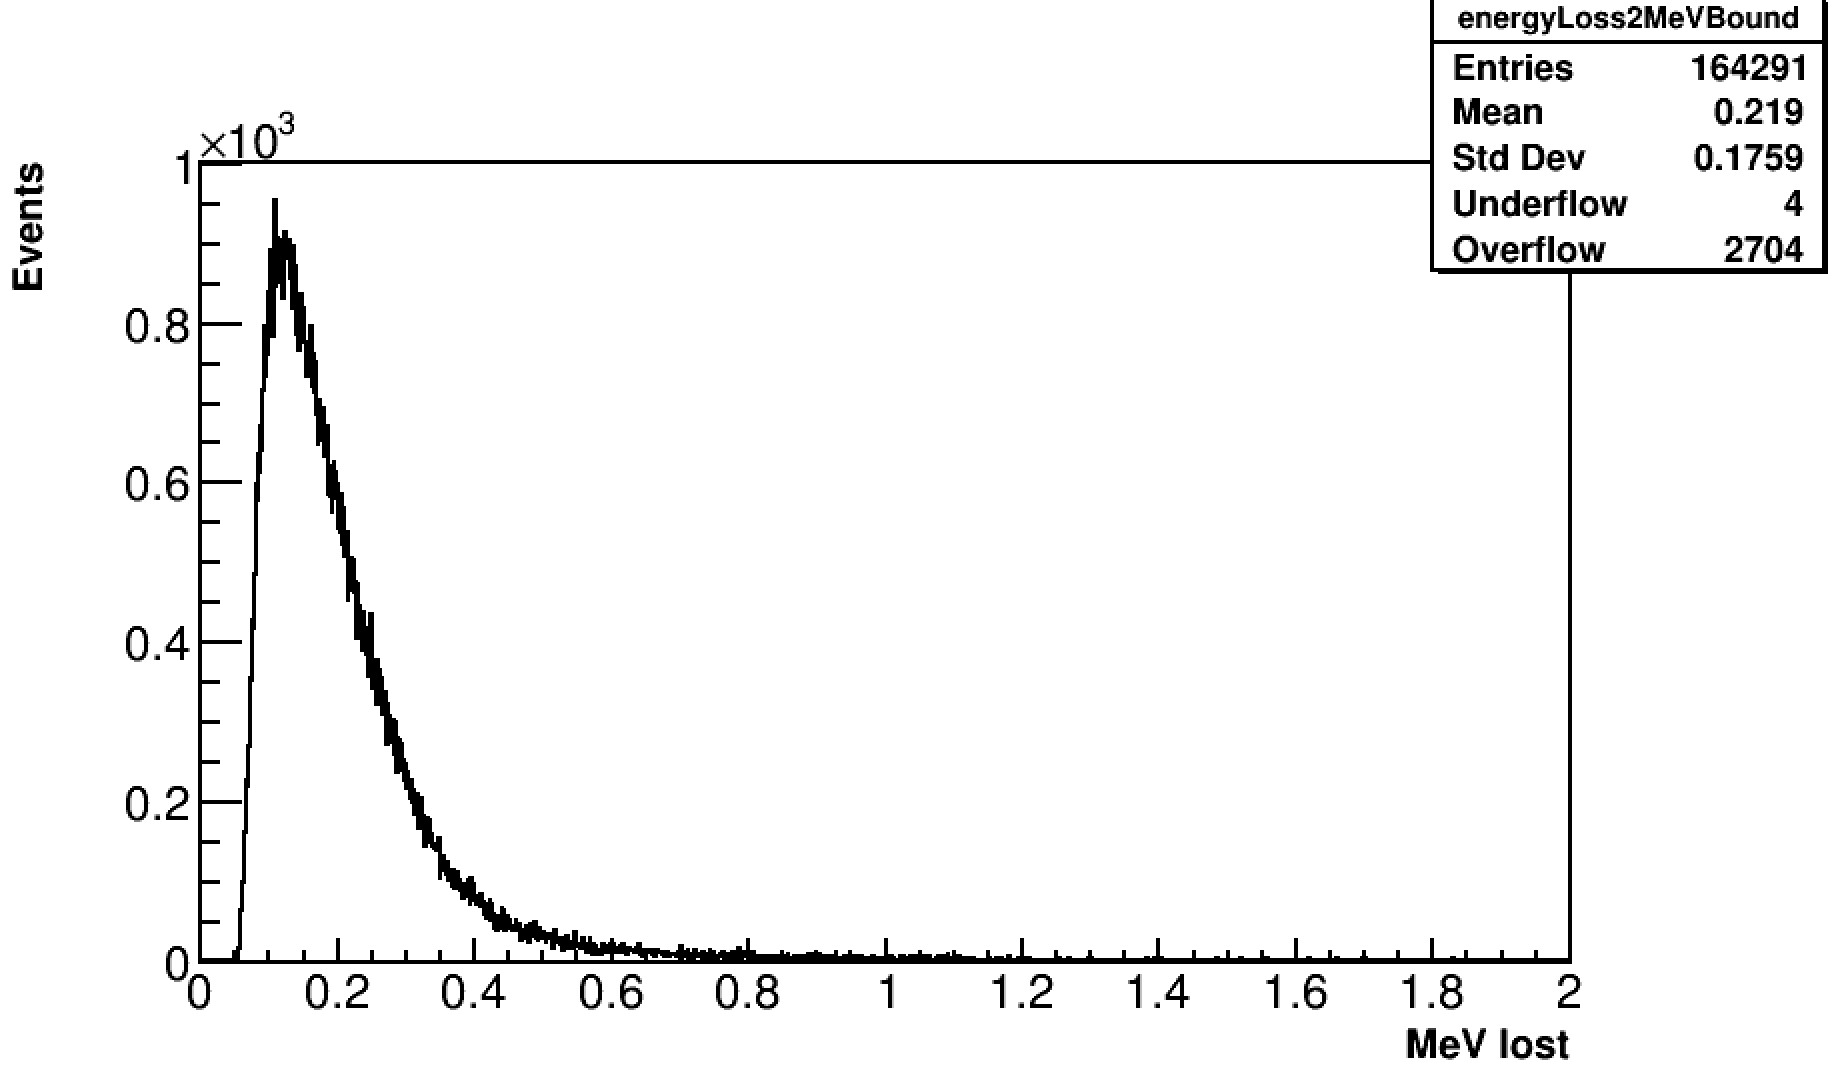
\includegraphics[width=1.0\textwidth]{eLoss}
\label{fig:eLoss}
\end{figure}
